\documentclass[12pt]{article}

\pagestyle{empty}
\setcounter{secnumdepth}{2}
%----------------------------------------------------------------------------------------
%   Packages and configurations
%----------------------------------------------------------------------------------------
\usepackage[dutch]{babel}
\usepackage{hyperref} %Allow for references
\usepackage{lastpage}
\usepackage{fancyheadings}
\hypersetup{
    colorlinks,
    citecolor=black,
    filecolor=black,
    linkcolor=black,
    urlcolor=black
} %Set up hyperlink colours.
\newcommand{\sectionbreak}{\clearpage} % Should start every section on its own page
\usepackage{geometry} % Required to change the page size to A4
\geometry{a4paper} % Set the page size to be A4 as opposed to the default US Letter
\usepackage{chngpage}
\usepackage{appendix}
%REMOVE IF HEADER/FOOTER BROKEN
\usepackage{fancyhdr} % Required for custom headers
\usepackage{extramarks} % Required for headers and footers
\usepackage{lastpage} % Required to determine the last page for the footer
%-----------------1
\topmargin=0cm
\oddsidemargin=0cm
\textheight=22.0cm
\textwidth=16cm
\parindent=0cm
\parskip=0.15cm
\topskip=0truecm
\raggedbottom
\abovedisplayskip=3mm
\belowdisplayskip=3mm
\abovedisplayshortskip=0mm
\belowdisplayshortskip=2mm
\normalbaselineskip=12pt
\normalbaselines
\usepackage{listings}
\usepackage[svgnames,table,xcdraw]{xcolor}
\lstset { 
    language=C,
    frame=single,
    escapeinside={\%*}{*)}, 
    breaklines=true,  
    backgroundcolor=\color{black!5},
    basicstyle=\footnotesize,
    commentstyle=\color{mygreen},
    numberstyle=\tiny\color{mygray},
    rulecolor=\color{black},
    keywordstyle=\color{blue},
}

\definecolor{mygreen}{rgb}{0,0.6,0}
\definecolor{mygray}{rgb}{0.5,0.5,0.5}
\definecolor{mymauve}{rgb}{0.58,0,0.82}
\usepackage{wasysym}
\pagestyle{fancy}
\lhead{Jim \textsc{van Abkoude} \& Julian G. \textsc{West}} % Top left header
\rhead{Opdrachten week 3} % Top center header
\lfoot{
\includegraphics[height=0.8cm]{avans}} % Bottom left footer
\cfoot{} % Bottom center footer
\rfoot{Pagina\ \thepage} % Bottom right footer
\renewcommand\headrulewidth{0.4pt} % Size of the header rule
\renewcommand\footrulewidth{0.4pt} % Size of the footer rule
\usepackage{graphicx} % Required for including pictures

\usepackage{float} % Allows putting an [H] in \begin{figure} to specify the exact location of the figure
\usepackage{wrapfig} % Allows in-line images such as the example fish picture
\usepackage{lipsum} % Used for inserting dummy 'Lorem ipsum' text into the template
\usepackage{pdfpages}
\usepackage[font={footnotesize}]{caption}
\graphicspath{{imgs/}}
\setlength\parindent{0pt} % Removes all indentation from paragraphs
%\usepackage{showframe}
\newcommand*{\SignatureAndDate}[1]{%
    \par\noindent\makebox[2.5in]{\hrulefill} \hfill\makebox[2.0in]{\hrulefill}%
    \par\noindent\makebox[2.5in][l]{#1}      \hfill\makebox[2.0in][l]{Date}%
}%Signature package
\begin{document}
\begin{titlepage}
\pagenumbering{Roman}
\newcommand{\HRule}{\rule{\linewidth}{0.5mm}} % Defines a new command for the horizontal lines, change thickness here

\center % Center everything on the page


\includegraphics[height=3cm]{avans}\\% Include a department/university logo - this will require the graphicx package
\textsc{\Large Avans Hogeschool Breda}\\[0.5cm] % Major heading such as course name
\textsc{\large Intelligente wireless sensornetwerken}\\[0.5cm] % Minor heading such as course title
\HRule \\[0.4cm]
{ \huge \bfseries Opdrachten week 3}\\[0.4cm] % Title of your document
\HRule \\[1.5cm]

\begin{minipage}{0.4\textwidth}
\begin{flushleft} \large
\emph{Auteurs:}\\
Jim \textsc{van Abkoude} \\
Julian \textsc{West} \\
\end{flushleft}
\end{minipage}
~
\begin{minipage}{0.4\textwidth}
\begin{flushright} \large
\emph{Docenten:} \\
Diederich \textsc{Kroeske} \\ % Supervisor's Name
Andries \textsc{van Dongen} \\ % Supervisor's Name
\end{flushright}
\end{minipage}\\[4cm]

{\large \today}\\[3cm] % Date, change the \today to a set date if you want to be precise

Versie: 0.1.0

\vfill % Fill the rest of the page with whitespace

\end{titlepage}

\clearpage
% \section*{Voorwoord}
% \addcontentsline{toc}{section}{Voorwoord}

% Guus Beckett \& Jim van Abkoude \\
% \today \\
% Breda
% \newpage
% \section*{Samenvatting}
% \addcontentsline{toc}{section}{Samenvatting}
% \lipsum[0-2]
% \newpage
% \tableofcontents
% \newpage
\pagenumbering{arabic}
\section{Setup}

De eerste taak met de XBee Serie 2 wireless radio modules was om de firmware te updaten/resetten. Er waren 5 Xbee modules aanwezig waarvan we 1 flashen met de coordinator AT firmware versie 20A7 en de anderen met de router AT firmware versie 22A7. We testen onze setup door met de coordinator XBee te transmitten en receiven in transparant modus en hetzelfde voor de router XBee. Jim stuurt ASCII data naar zijn XBee die deze via Zigbee verstuurt naar de XBee aan Julian's laptop is gekoppeld en via UART komt de data in de terminal terug. Figuur~\ref{fig:setup1} laat de route zien en figuur~\ref{fig:output1} en~\ref{fig:output2} de output in een terminal.\\
Verder hebben we de adressen van de XBee modules in tabel~\ref{tab:info1} genoteerd. \\
\begin{center}
\begin{figure}[h]
\includegraphics[scale=.25]{test_setup_1.jpg}
\caption{Initiële test setup}
\label{fig:setup1}
\end{figure}
\end{center}
\begin{center}
\begin{figure}[h]
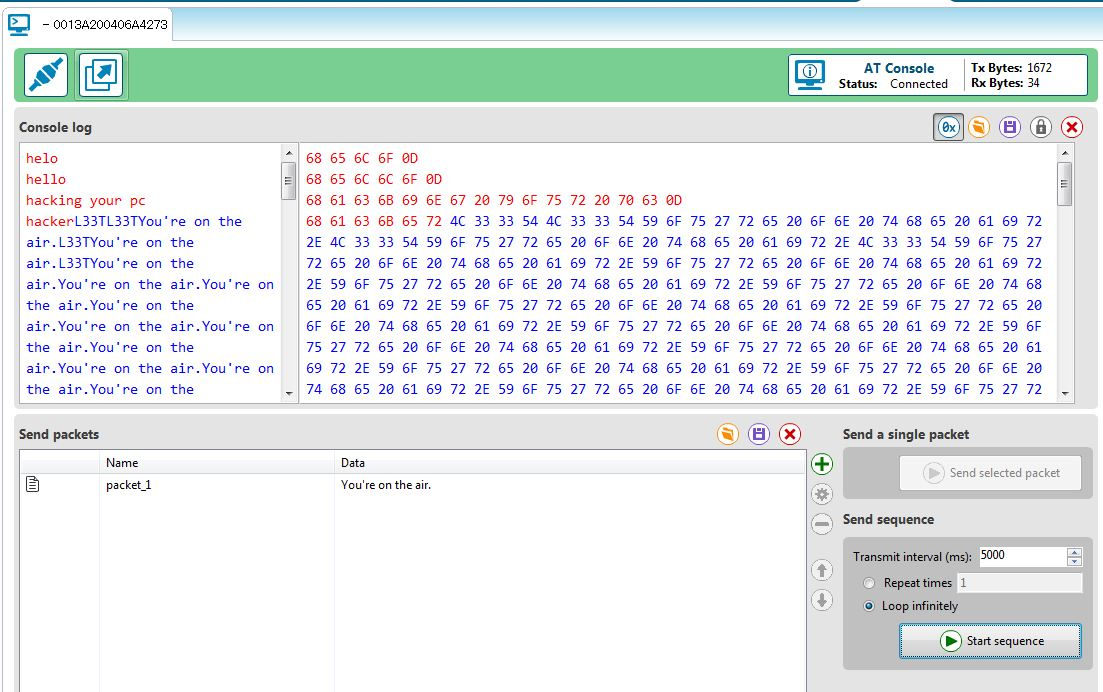
\includegraphics[scale=.6]{Serial_Capture.jpg}
\caption{Capture van data transfer in XCTU-NG}
\label{fig:output1}
\end{figure}
\end{center}
\clearpage
\begin{center}
\begin{figure}[h]
\includegraphics[scale=.8]{Terminal_Output.jpg}
\caption{Capture van data transfer in Hercules}
\label{fig:output2}
\end{figure}
\end{center}
\begin{table}[h]
\begin{center}
\begin{tabular}{ll}
\rowcolor[HTML]{656565} 
\textbf{Type} & \textbf{64-bit adres} \\
Co\"{o}rdinator   & ...40A20C86           \\
Router        & ...406A4273           \\
Router A      & ...40A20CC8           \\
Router B      & ...408B183C           \\
Router C      & ...406A4282                      
\end{tabular}
\end{center}
\caption{Tabel van XBee modules en hun (lage) 64-bit adres}
\label{tab:info1}
\end{table}
\clearpage
\section{Opdrachten}
\subsection*{Opdracht 1a}
In onze setup hebben we grotendeels de opdracht uitgevoerd. We hadden niet de bestemming adres ingesteld tijdens onze initi\"{e}le setup. Nadat we het adres van de coordinator op de router programeerde en vice versa, was de communicatie weer mogelijk. De chat verliep zoals in figuur~\ref{fig:output3}.\\
\begin{center}
\begin{figure}[h]
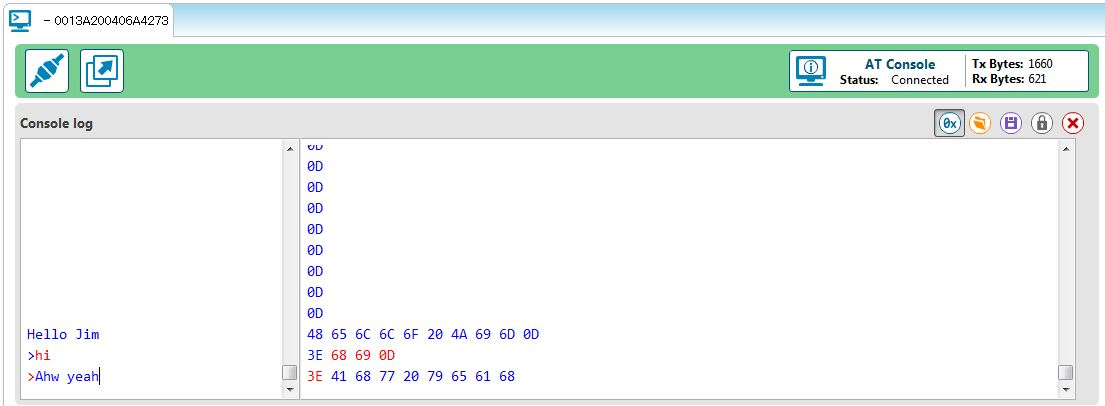
\includegraphics[scale=1]{Serial_Capture_2.jpg}
\caption{Capture van data transfer in XCTU-NG met andere settings}
\label{fig:output3}
\end{figure}
\end{center}
\clearpage
\subsection*{Opdracht 1b}
Als eerste zetten we een test setup op met 3 XBee. Deze is in figuur~\ref{fig:setup2} te bewonderen. In dit diagram wordt de data broadcasting weergeven vanaf de coordinator. De a en b operaties gebeuren niet synchroon.\\
Omdat 0 schrijven in XCTU-NG niet werkt, moesten we even via de terminal direct ATDL0 instellen. \\
Nadat we ATDL \& ATDH op de routers op 0 zetten en voor de co\"{o}rdinator ATDL op 0xFFFF \& ATDH op 0, was de communicatie succesvol. De coordinator stuurt een bericht naar alle Zigbee luisterende devices met PAN id 4016 en de routers sturen naar alleen de co\"{o}rdinator. Het bewijs is te zien in figuren~\ref{fig:output4} tot~\ref{fig:output6}
\begin{center}
\begin{figure}[h]
\includegraphics[scale=.25]{test_setup_2.jpg}
\caption{Test setup voor 3 XBee modules}
\label{fig:setup2}
\end{figure}
\end{center}
\begin{center}
\begin{figure}[h]
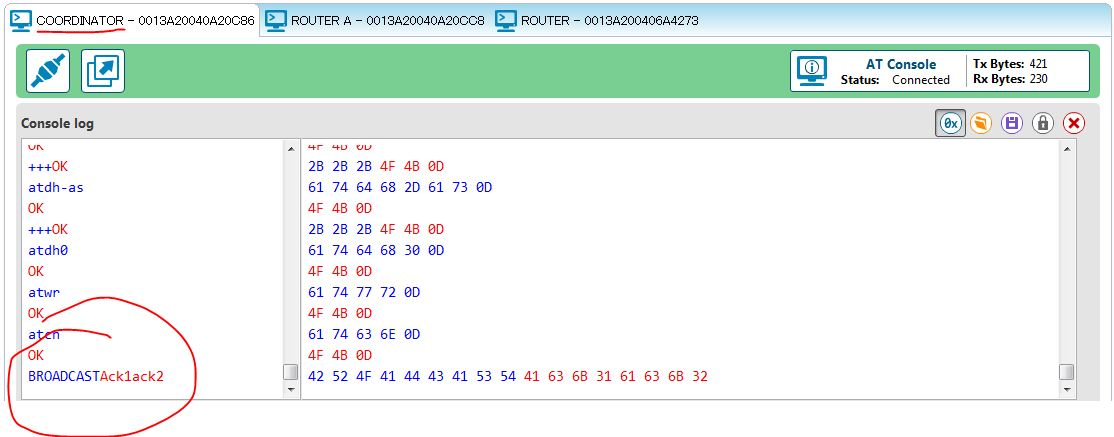
\includegraphics[scale=.7]{coord_capture.jpg}
\caption{Terminal capture van de co\"{o}rdinator}
\label{fig:output4}
\end{figure}
\end{center}
\begin{center}
\begin{figure}[h]
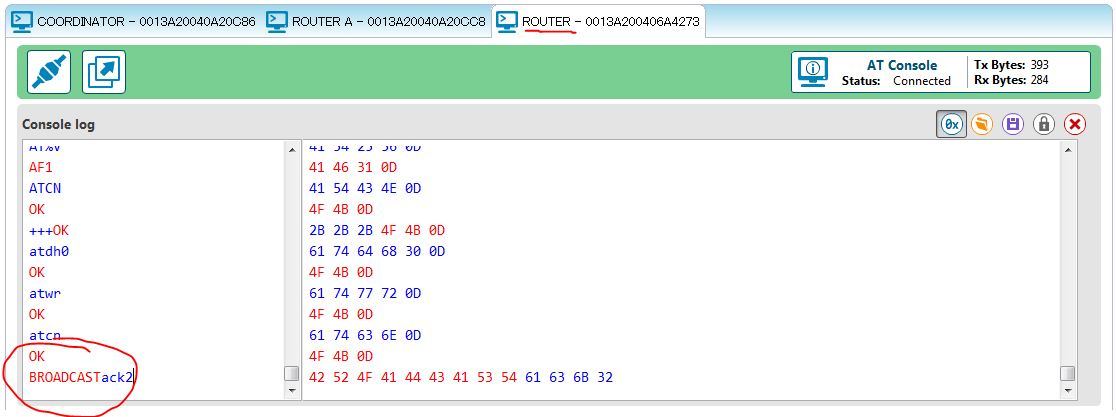
\includegraphics[scale=.7]{rout_capture.jpg}
\caption{Terminal capture van de letterloze router}
\label{fig:output5}
\end{figure}
\end{center}
\begin{center}
\begin{figure}[h]
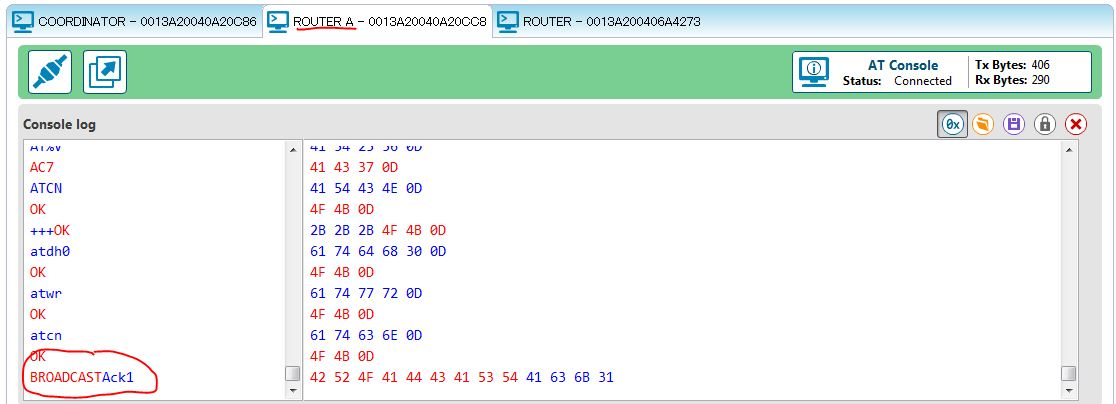
\includegraphics[scale=.7]{routA_capture.jpg}
\caption{Terminal capture van router A}
\label{fig:output6}
\end{figure}
\end{center}
\clearpage
%\subsection*{Opdracht 1c}
%Als laatste hebben we de XBee via de Arduino uitgelezen en aangestuurd.
%Dit komt later.

\end{document}
